% Capítulo 9 – gerado a partir do relatório; edite livremente
\begin{landscape}

\chapter{FOLHA DE PROCESSO}

{\scriptsize\renewcommand{\arraystretch}{1.25}
\captionof{quadro}{Folha de processo da engrenagem}\label{quad:folha}
\begin{longtable}{|>{\centering\arraybackslash}p{\dimexpr 0.0391\linewidth-2\tabcolsep\relax}|>{\raggedright\arraybackslash}p{\dimexpr 0.0738\linewidth-2\tabcolsep\relax}|>{\raggedright\arraybackslash}p{\dimexpr 0.1953\linewidth-2\tabcolsep\relax}|>{\raggedright\arraybackslash}p{\dimexpr 0.1432\linewidth-2\tabcolsep\relax}|>{\raggedright\arraybackslash}p{\dimexpr 0.1128\linewidth-2\tabcolsep\relax}|>{\raggedright\arraybackslash}p{\dimexpr 0.1909\linewidth-2\tabcolsep\relax}|>{\raggedright\arraybackslash}p{\dimexpr 0.0694\linewidth-2\tabcolsep\relax}|>{\raggedright\arraybackslash}p{\dimexpr 0.0998\linewidth-2\tabcolsep\relax}|>{\centering\arraybackslash}p{\dimexpr 0.0607\linewidth-2\tabcolsep\relax}|}
\hline
\rowcolor{cinza} \textbf{Nº} & \textbf{Equipamento} & \textbf{Descrição da operação} & \textbf{Fixação e referências} & \textbf{Croqui} & \textbf{Parâmetros de corte} & \textbf{Ferramenta} & \textbf{Máquina-ferramenta} & \textbf{Tempo de corte (min)} \\ \hline \endfirsthead
\hline
\rowcolor{cinza} \textbf{Nº} & \textbf{Equipamento} & \textbf{Descrição da operação} & \textbf{Fixação e referências} & \textbf{Croqui} & \textbf{Parâmetros de corte} & \textbf{Ferramenta} & \textbf{Máquina-ferramenta} & \textbf{Tempo de corte (min)} \\ \hline \endhead
10 & Bancada & Inspeção do bruto Ø160 $\times$ 58 mm: diâmetro, comprimento, dureza e certificado & – & 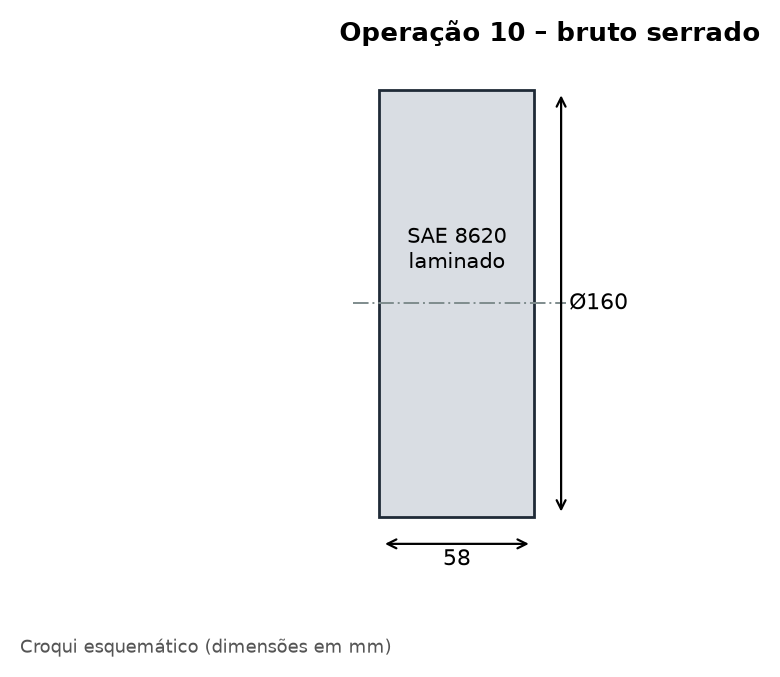
\includegraphics[width=2.2cm]{figuras/croqui_op10.png} & – & Paquímetro e durômetro & – & 3,0 \\ \hline
20.1 & Torno CNC & Facear a face A em 2 passes de desbaste & Placa de 3 castanhas duras no Ø160, pega de 15 mm & 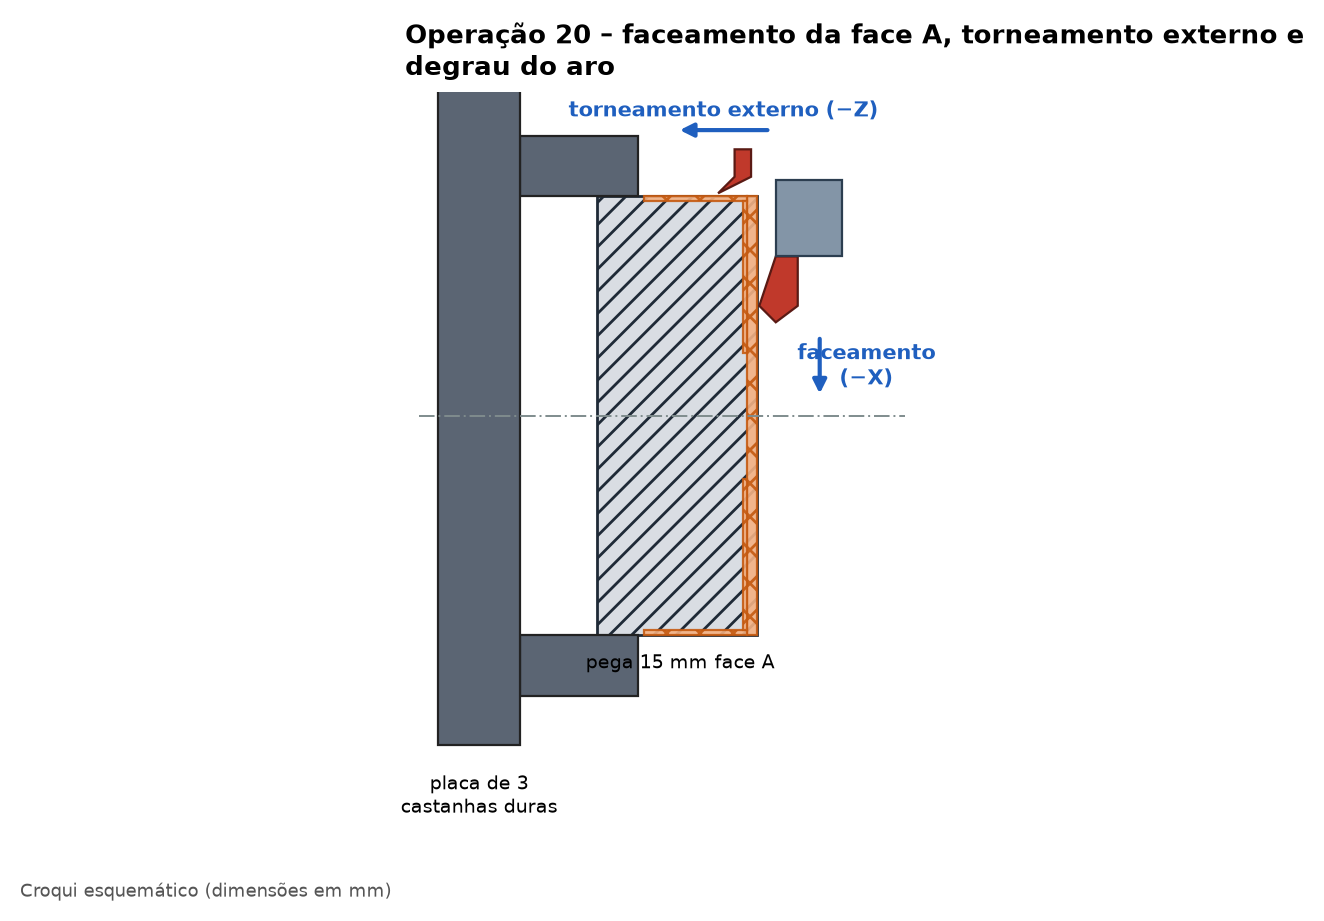
\includegraphics[width=2.2cm]{figuras/croqui_op20a.png} & a\textsubscript{p} = 1,425 mm; f = 0,22 mm; v\textsubscript{c} = 300 m/min; n = 597 a 3.000 rpm & T01 & ROMI Centur 30D & 0,66 \\ \hline
20.2 & Torno CNC & Tornear Ø160 para Ø157 em 36 mm & Idem &  & a\textsubscript{p} = 1,5 mm; f = 0,22 mm; v\textsubscript{c} = 280 m/min; n = 557 rpm & T01 & Idem & 0,31 \\ \hline
20.3 & Torno CNC & Rebaixar a face do aro 1,65 mm (ressalto do cubo) & Idem &  & a\textsubscript{p} = 1,15 mm; f = 0,22 mm; v\textsubscript{c} = 300 m/min & T01 & Idem & 0,28 \\ \hline
20.4 & Torno CNC & Acabar face do cubo, Ø46 com chanfro de 2 mm, face do aro e Ø156 & Idem &  & a\textsubscript{p} = 0,5 mm; f = 0,15 mm; v\textsubscript{c} = 400 m/min & T02 & Idem & 0,67 \\ \hline
20.5 & Torno CNC & Furar Ø23 passante & Idem & 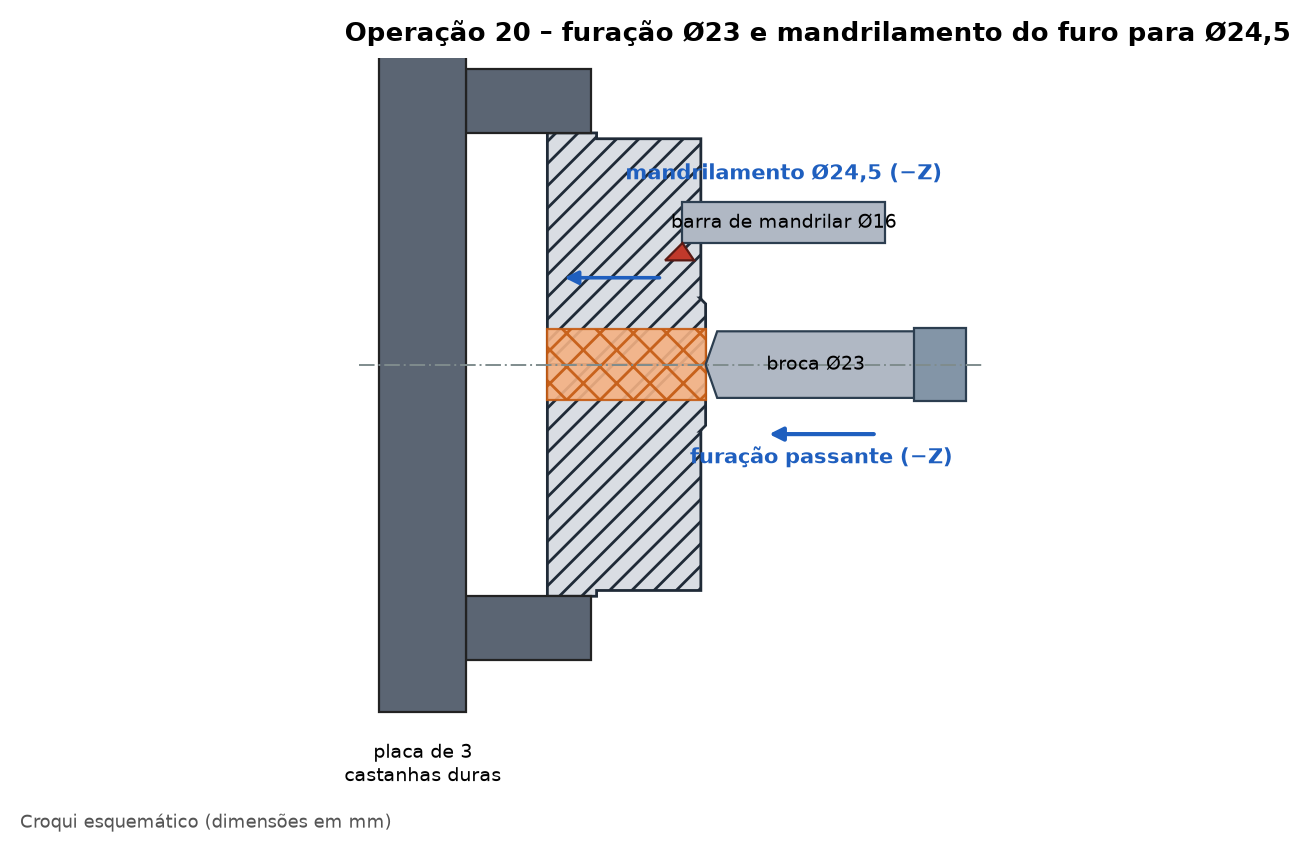
\includegraphics[width=2.2cm]{figuras/croqui_op20b.png} & f = 0,09 mm; v\textsubscript{c} = 150 m/min; n = 2.076 rpm & T03 & Idem & 0,31 \\ \hline
20.6 & Torno CNC & Mandrilar o furo para Ø24,5 e chanfrar 0,5 $\times$ 45° & Idem &  & a\textsubscript{p} = 0,75 mm; f = 0,10 mm; n = 3.000 rpm & T04 & Idem & 0,20 \\ \hline
20.7 & Torno CNC & Usinar o rebaixo da face A (Ø46 a Ø110, prof. 17 mm, raios R3) e quebrar arestas & Idem & 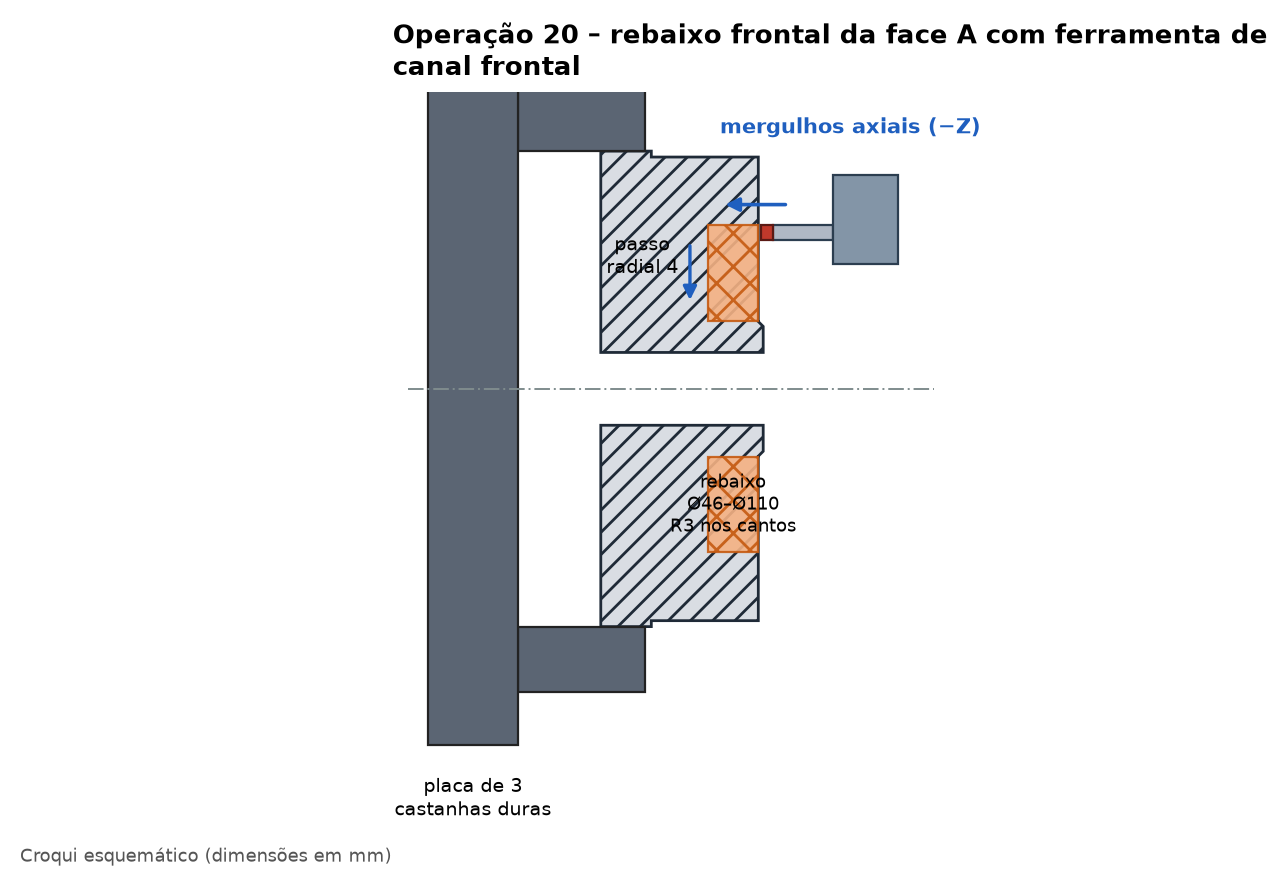
\includegraphics[width=2.2cm]{figuras/croqui_op20c.png} & f = 0,07 mm; v\textsubscript{c} = 160 m/min; n = 485 a 999 rpm & T05 e T02 & Idem & 4,18 \\ \hline
30.1 & Torno CNC & Facear a face B até o cubo com 51,3 mm e rebaixar a face do aro & Castanhas moles no Ø156; face A no anel de encosto & 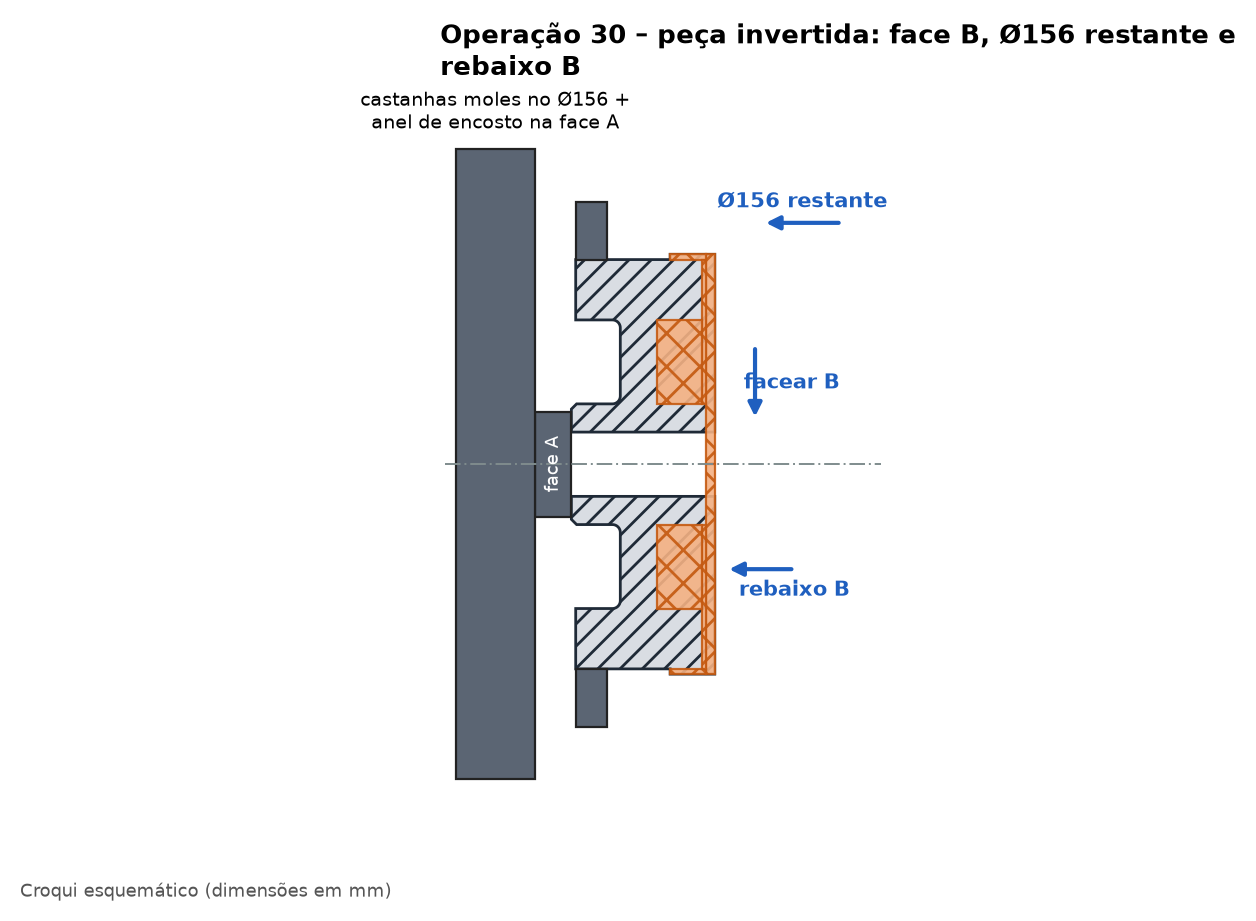
\includegraphics[width=2.2cm]{figuras/croqui_op30.png} & Como em 20.1 e 20.3 & T01 & ROMI Centur 30D & 0,87 \\ \hline
30.2 & Torno CNC & Tornear os 16 mm restantes do Ø156 e acabar o lado B & Idem &  & Como em 20.2 e 20.4 & T01 e T02 & Idem & 0,63 \\ \hline
30.3 & Torno CNC & Usinar o rebaixo da face B e chanfrar & Idem &  & Como em 20.7 & T05, T02 e T04 & Idem & 4,18 \\ \hline
40 & Fresadora universal & Fresar os 24 dentes: desbaste com 12,6 mm e acabamento com 13 mm de profundidade; divisão de 15° & Mandril Ø24,5 com encosto na face A, entre cabeçote divisor e contraponta & 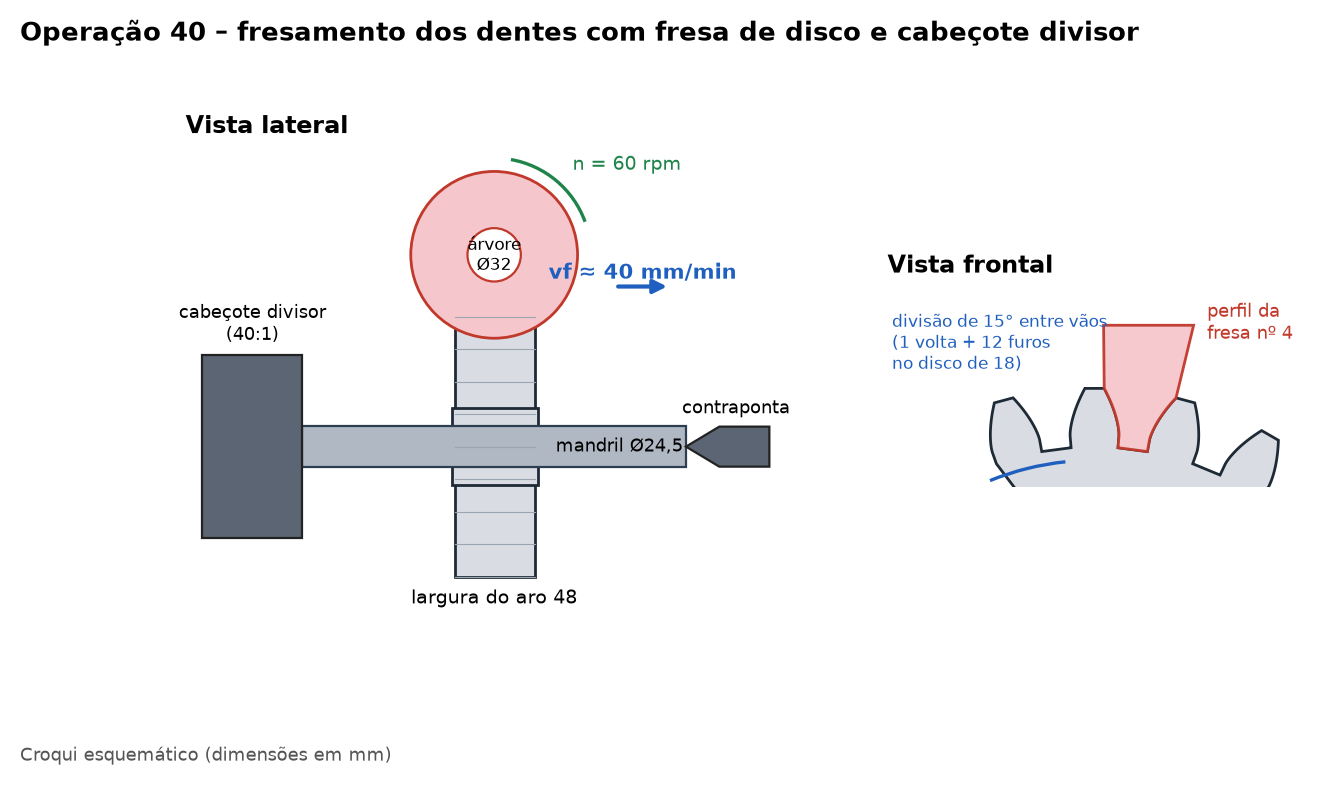
\includegraphics[width=2.2cm]{figuras/croqui_op40.png} & n = 60 rpm; f\textsubscript{z} = 0,055 mm; v\textsubscript{f} = 40 mm/min; óleo integral & F01 & KNUTH UWF 5 com divisor UT & 104,7 \\ \hline
50 & Centro de usinagem & Fresar os 4 rasgos em arco (R30 a R48, extremidades R9), passantes na alma & Pino Ø24,5, apoio na face do cubo, porca e arruela & 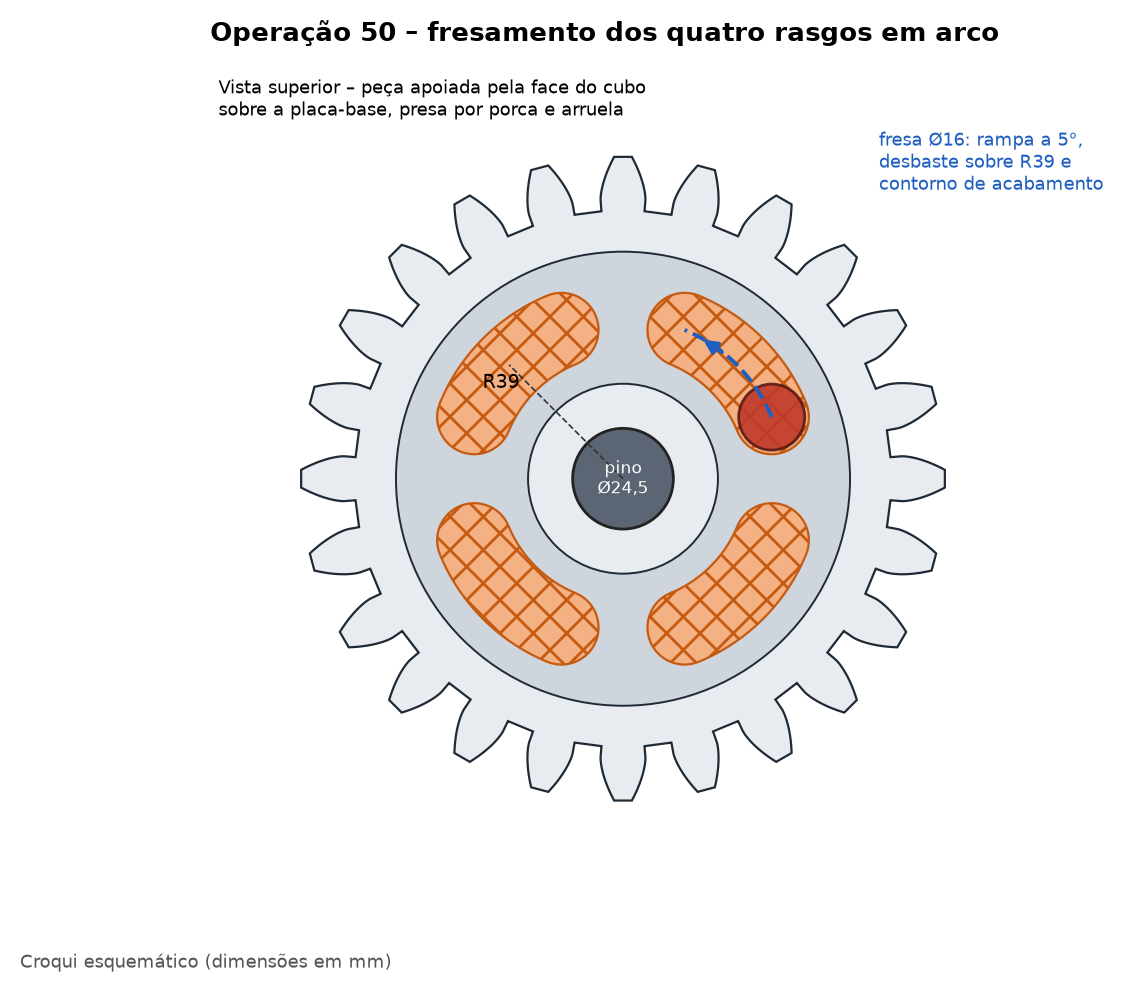
\includegraphics[width=2.2cm]{figuras/croqui_op50.png} & n = 5.471 rpm; f\textsubscript{z} = 0,10 e 0,20 mm; a\textsubscript{p} = 5 mm; a seco & F02 & ROMI D 800 & 1,33 \\ \hline
60 & Prensa hidráulica & Brochar o rasgo de chaveta de 8 mm com fundo a 16 mm do eixo (2 passes) & Bucha-guia no furo; pino em um rasgo em arco & 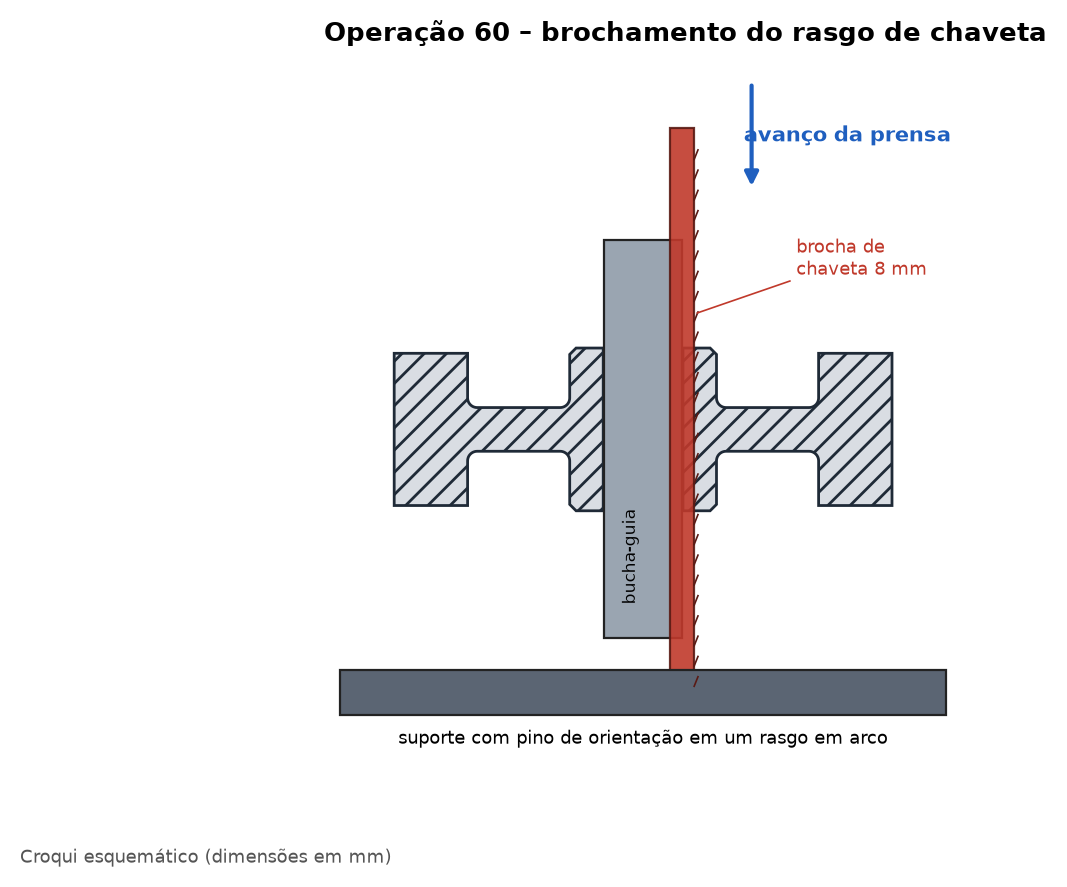
\includegraphics[width=2.2cm]{figuras/croqui_op60.png} & v $\approx$ 3 m/min; óleo integral & B01 & Prensa de 5 tf & 0,23 \\ \hline
70 & Bancada & Rebarbar e medir sobre 3 dentes (46,30 mm) & – & 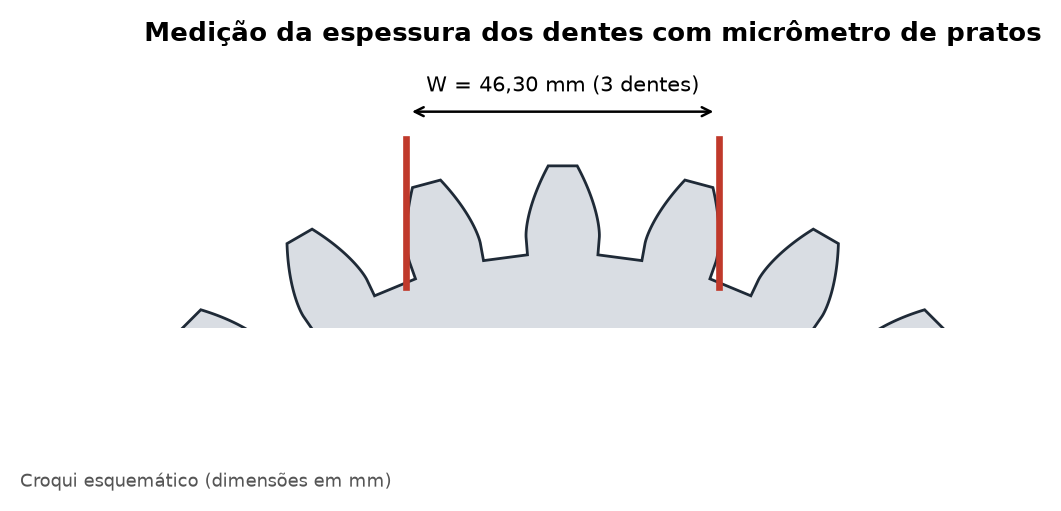
\includegraphics[width=2.2cm]{figuras/croqui_op110.png} & – & Limas; micrômetro de pratos & – & 20,0 \\ \hline
80 & Fornecedor & Cementar, temperar e revenir (58 a 62 HRC) & – &  & – & – & Forno de cementação & – \\ \hline
90 & Retificadora plana & Retificar as faces do cubo até 51,00 mm e desmagnetizar & Mesa magnética, apoio na face oposta do cubo & 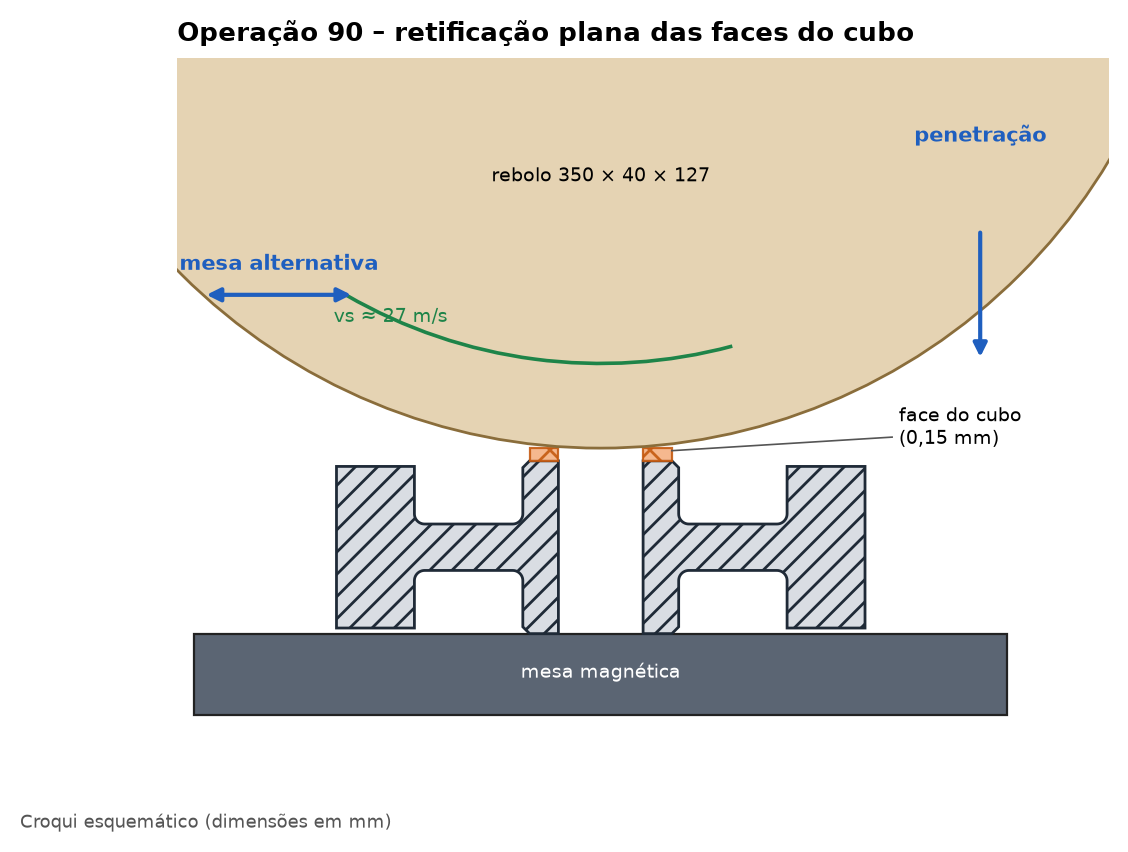
\includegraphics[width=2.2cm]{figuras/croqui_op90.png} & v\textsubscript{s} = 26,6 m/s; v\textsubscript{w} = 15 m/min; s = 8 mm; a\textsubscript{e} = 0,02 e 0,005 mm & R01 & KNUTH HFS 3063 & 2,53 \\ \hline
100 & Retificadora interna & Retificar o furo para Ø25 H7 & Placa de roletes no diâmetro primitivo; encosto na face A & 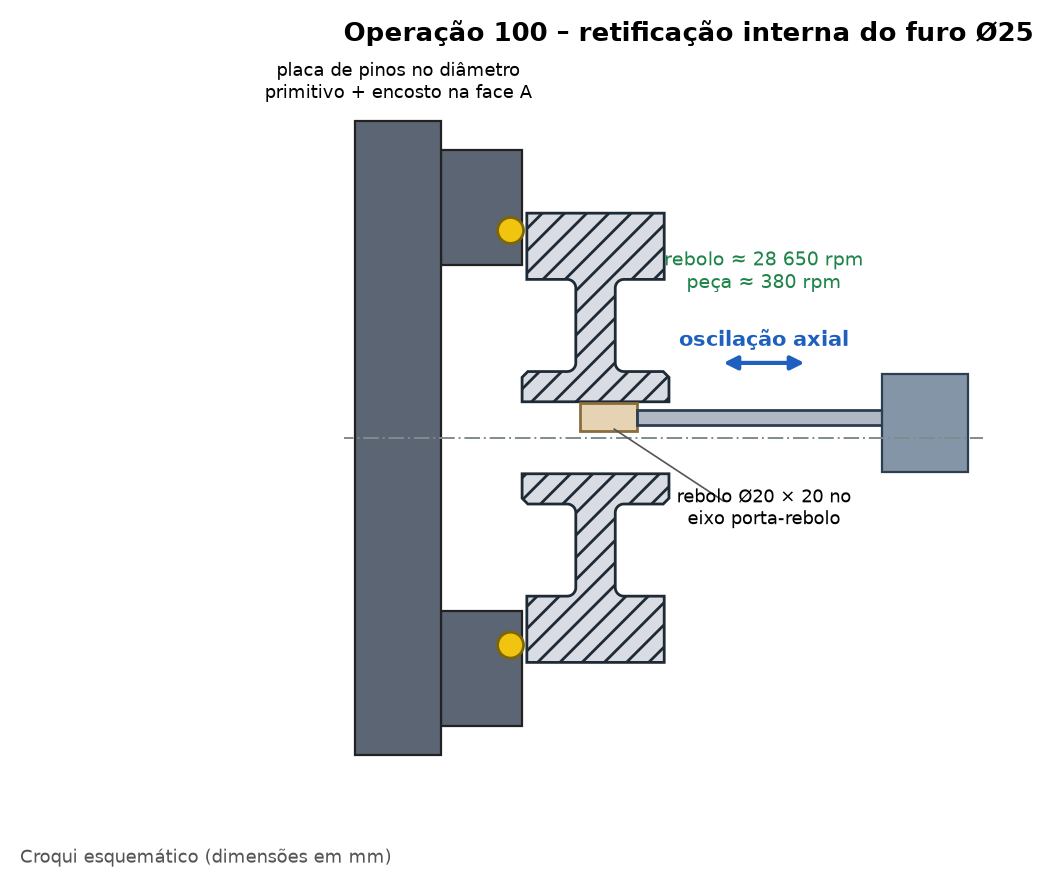
\includegraphics[width=2.2cm]{figuras/croqui_op100.png} & v\textsubscript{s} = 30 m/s; n\textsubscript{w} = 382 rpm; a\textsubscript{e} = 0,005 e 0,0025 mm & R02 & STUDER S121 & 0,88 \\ \hline
110 & Metrologia & Inspeção final: furo, comprimento do cubo, medida sobre dentes, batimento, dureza e rugosidade & – &  & – & Calibrador tampão, súbito, rugosímetro, durômetro & – & 15,0 \\ \hline
\end{longtable}}
\fonte{Elaborado pelos autores.}


\end{landscape}
